% PP-Article.tex for AEA last revised 22 June 2011
\documentclass[twocolumn, a4paper]{article}

%\usepackage{amsmath}
\usepackage[dutch]{babel}
\usepackage{subcaption}
\usepackage[width=.8\textwidth]{caption}
\usepackage{float}
\usepackage{booktabs}
\usepackage{multicol}
\usepackage{minted}
% If you have trouble with the mathtime package please see our technical support 
% document at: http://www.aeaweb.org/templates/technical_support.pdf
% You may remove the mathtime package if you can't get it working but your page
% count may be inaccurate as a result.
% \usepackage[cmbold]{mathtime}
\usepackage{xargs}                      % Use more than one optional parameter in a new commands
\usepackage[pdftex,dvipsnames]{xcolor}  % Coloured text etc.
% 
\usepackage{pdfpages}
\usepackage[colorinlistoftodos,prependcaption,textsize=tiny]{todonotes}
\newcommandx{\unsure}[2][1=]{\todo[linecolor=red,backgroundcolor=red!25,bordercolor=red,#1]{#2}}
\setlength{\marginparwidth}{2cm}
% Note: you may use either harvard or natbib (but not both) to provide a wider
% variety of citation commands than latex supports natively. See below.

% Uncomment the next line to use the natbib package with bibtex 
%\usepackage{natbib}
\usepackage{titlesec}

%\titlespacing*\section{0pt}{12pt plus 4pt minus 2pt}{0pt plus 2pt minus 2pt}
%\titlespacing*\subsection{0pt}{12pt plus 4pt minus 2pt}{0pt plus 2pt minus 2pt}
%\titlespacing*\subsubsection{0pt}{12pt plus 4pt minus 2pt}{0pt plus 2pt minus 2pt}

% Uncomment the next line to use the harvard package with bibtex`
%\usepackage[abbr]{harvard}

% This command determines the leading (vertical space between lines) in draft mode
% with 1.5 corresponding to "double" spacing.
\begin{document}

\title{Geavanceerde computerarchitectuur: Labo 03 \\ 
\large{Parallel computing via Raspberry Pi's}}
\author{\textsc{Anton Danneels en Pieter Delobelle}}
\date{}
\maketitle

\section{Inleiding}

\section{Analyse}
Deze sectie zal ingaan op de gebruikte technieken en relevante concepten. Het eerste concept is dat van \emph{message brokers}, wat in Subsectie~\ref{ss:broker} wordt uitgediept. Hierna wordt ingegaan op hoe dit gebruikt kan worden in de context van gedistribueerde stream-verwerking in Subsectie~\ref{ss:stream}. Tenslotte wordt \emph{Docker Swarm} bekeken in Subsectie~\ref{ss:swarm}.

\subsection{Message brokers}\label{ss:broker}
Een \emph{message broker} kadert in \emph{message-oriented middleware}, waarbij applicaties asynchroon data kunnen sturen en ontvangen. Hierbij sturen alle applicaties berichten naar een \emph{broker}, die deze berichten dan weer doorstuurt.

\begin{figure}[htb]
    \centering
    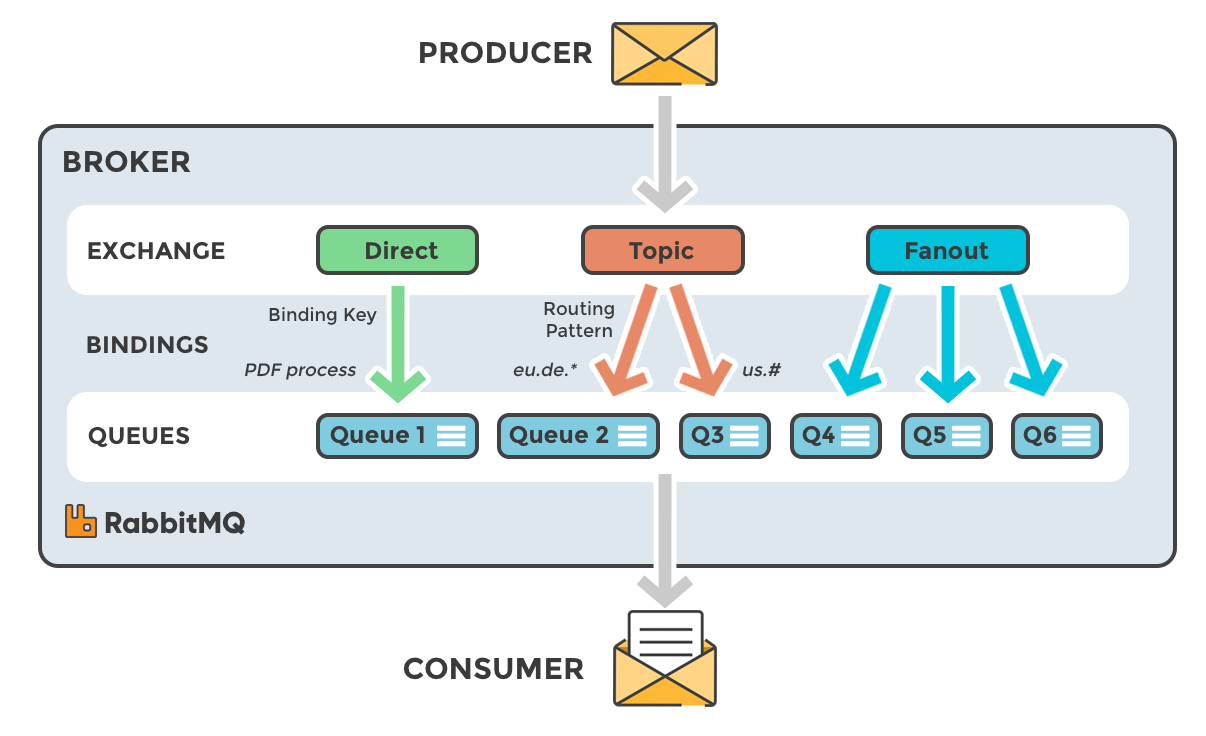
\includegraphics[width=0.43\textwidth]{exchanges-topic-fanout-direct.png}
    \caption{Illustratie van een \emph{message broker}.}\label{fig:broker}
\end{figure}

De applicaties die berichten produceren worden \emph{producers} genoemd en de applicaties die ze consumeren noemen \emph{consumers}. De producers sturen berichten naar een \emph{exchange} op de broker. Op basis van een criterium worden deze berichten dan doorgestuurd naar een wachtrij (\emph{queue}) op de broker, waarop een consumer zich kan abonneren.

Het gebruik van een broker heeft enkele voordelen. Zo is er een ontkoppeling van applicaties; er zijn dus geen directe connecties nodig. Vooral de setup is hierdoor eenvoudiger. 

Ook is er automatisch een vorm van \emph{load balancing}, aangezien meerdere consumers zich kunnen abonneren op een gedeelde wachtrij. Mocht een consumer uitvallen, kunnen de andere consumers dit automatisch opvangen. 

In dit geval wordt RabbitMQ gebruikt. Dit is een \emph{polyglot broker}, wat een mooie uitdrukking is om aan te geven dat meerdere protocollen ondersteund worden, zoals MQTT, AMQP en WebSTOMP.

\subsection{Stream-verwerking}\label{ss:stream}
\emph{Stream processing} is een veelgebruikte architectuur voor operaties uit te voeren op een stroom van data. In een gedistribueerde context zijn hier systemen voor zoals Heron. Hierbij voeren operatoren allemaal kleine operaties uit, waarbij de voorkeur wordt gegeven aan atomaire staatloze operaties.

Om operatoren met elkaar te verbinden, kan een systeem zoals in Figuur~\ref{fig:operator-queue} gebruikt worden. Hierbij stuurt iedere operator een bericht met een vooraf vastgelegde \emph{topic ID}. Iedere operator abonneert zich dan ook op een vooraf vastgelegde queue, of maakt deze aan mocht die nog niet bestaan. 

\begin{figure}[htb]
    \centering
    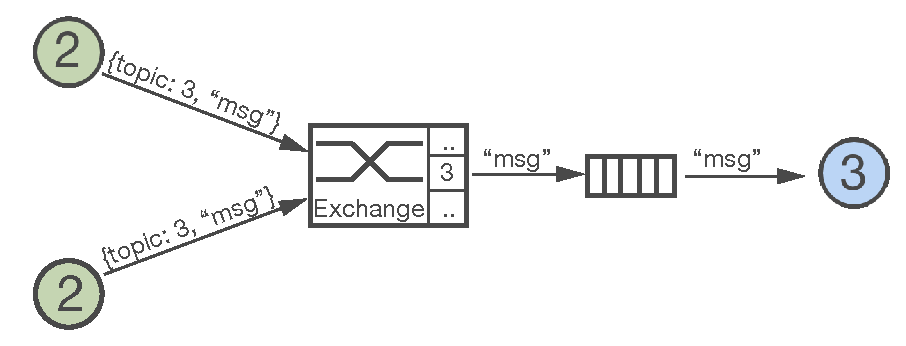
\includegraphics[width=0.43\textwidth]{operator_queue}
    \caption{Illustratie van hoe een broker\\tussen operators geïntegreerd zit.}\label{fig:operator-queue}
\end{figure}

\begin{figure*}[htb]
    \centering
    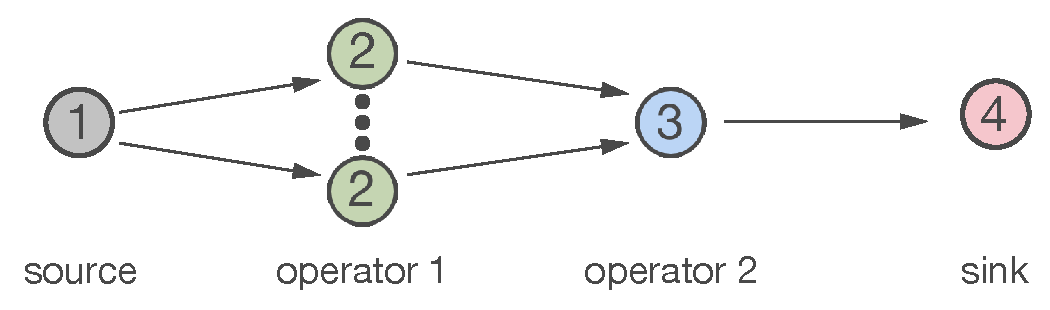
\includegraphics[width=0.63\textwidth]{flow}
    \caption{Topologie van deze \emph{stream}, waarbij operator 1 dynamisch geschaald wordt.}\label{fig:flow}
\end{figure*}


\subsection{Docker Swarm}\label{ss:swarm}
Docker is een technologie die het mogelijk maakt om applicaties in \emph{containers} uit te voeren. Het doel van deze containers is om de illusie op te wekken dat deze applicaties op een apart besturingssysteem draaien. Hierdoor is het mogelijk om alleen de benodigde software te installeren. Docker Swarm is een technologie bovenop Docker die het mogelijk maakt om automatisch containers uit te voeren op een collectie van apparaten.

Er zijn twee soorten nodes, managers en workers. Managers zullen automatisch werkers uitkiezen waar containers op moeten draaien. Daarnaast heeft Docker Swarm features zoals automatische \emph{load balancing} en \emph{container registries}, waardoor nodes in de swarm hun container kunnen downloaden van een manager.

\section{Oplossing}

\subsection{Operatie}
De reken-intensieve operatie die door verschillende Raspberry Pi's gaat uitgevoerd worden, is het ontbinden van een getal in priemfactoren. Tot op heden is hier geen efficiënt algoritme voor gevonden.

\subsection{Architectuur}
In de architectuur van het systeem zitten vier operatoren:

\begin{enumerate}
    \item \textbf{Source}: een nummer-generator die getallen genereert tussen 1 en 10 000 000 met een vaste frequentie $f=20$ Hz.
    \item \textbf{Operatie 1}: Ontbinden van deze getallen in een priemfactoren. Deze operatie is een transformatie op de data, daarom gebruiken we verder \emph{transform} als naam van deze operatie.
    \item \textbf{Operatie 2}: Samenvoegen van de array van priemfactoren naar een leesbare tekst.
    \item \textbf{Sink}: Consumeren van alle teksten, deze voorzien van een timestamp en opslaan naar een bestand. 
\end{enumerate}

Aangezien het ontbinden in priemfactoren vermoedelijk  de \emph{bottleneck} zal zijn, zal deze operatie incidenteel geschaald worden. Deze topologie is ook te zien in Figuur~\ref{fig:flow}.

\subsection{Implementatie}
Een van de voordelen is dat het systeem agnostisch wat betreft de programmeertaal en besturingssysteem. De twee operaties zitten beiden in Docker-containers, waardoor het onderliggende besturingssysteem niet uitmaakt. 

Wat betreft de programmeertaal, kan iedere programmeertaal die JSON kan parsen gebruikt worden. Dit is namelijk het formaat waarin de berichten beschreven worden. Een tweede voorwaarde is dat een van de volgende protocollen ondersteunt moet worden:
\begin{itemize}
    \item MQTT
    \item AMQP 0.x
    \item AMQP 1.x
    \item HTTP
    \item Stomp over WebSockets (WebSTOMP)
\end{itemize}

Beide operaties worden in JavaScript geschreven, wat vanuit de node.js \emph{runtime} aangeroepen wordt. Hierbij wordt Er gebruik gemaakt van een AMQP-bibliotheek. De code voor beide operatoren is te vinden in de appendices. 

Het zal opvallen dat de implementatie van beide operatoren zeer gelijkaardig is. Er zitten slechts enkele verschillen:

\begin{itemize}
    \item \textbf{Operatie}: het spreekt voor zich dat bij een andere operator er ook daadwerkelijk een andere operatie uitgevoerd wordt. Voor een transformatie is dit een functie met een functie die één argument neemt en één output genereert. Voor een filter-operatie zal er één of geen output gegeneerd worden.
    \item \textbf{Naam huidige operator}: Om zichzelf te kunnen abonneren op een wachtrij, is het noodzakelijk om een unieke ID van de huidige operatie te hebben. In dit geval is deze \emph{hardcoded}, aangezien er maar twee operators zijn.
    \item \textbf{Naam volgende operator}: Om de berichten te kunnen routen naar de volgende operator, moet er een \emph{topic ID} meegegeven worden. Deze ID is ook \emph{hardcoded}, wegens het kleine aantal operatoren. 
\end{itemize}

Om een volledig, dynamisch systeem te definiëren, zou een generieke operator geschreven kunnen worden. Deze drie parameters kunnen dan opgeslagen in een extern bestand, waarom een enkele parameter bepaalt wat de rol van de operator wordt. 

Wat betreft de \emph{source}- en \emph{sink}-operatoren, wordt er gekozen voor een implementatie in Python. Deze systemen zitten niet in een Docker-container, aangezien dit in een reëele situatie ook niet het geval zal zijn. De code voor beide systemen is te vinden in de appendices.

Om het aantal operatoren te schalen, wordt gebruik gemaakt van de schaal-functionaliteit van Docker Swarm. Dit systeem verdeelt alle operatoren automatisch over de nodes in de swarm.
 
\begin{minted}{console}
    docker service scale <ID>=<NR>
\end{minted}

In Appendix~\ref{appendix:schalen} is het resultaat van zo'n operatie weergegeven. 

Daarnaast is de broker, RabbitMQ, op een van de Raspberry Pi's gehost. Eveneens in een Docker container. Deze container kan opgezet worden met de volgende Dockerfile.  

\begin{minted}{docker}
FROM rabbitmq

RUN rabbitmq-plugins enable 
    --offline rabbitmq_management
RUN rabbitmq-plugins enable 
    --offline rabbitmq_stomp
RUN rabbitmq-plugins enable
    --offline rabbitmq_web_stomp
RUN rabbitmq-plugins enable 
    --offline rabbitmq_amqp1_0

EXPOSE 15671 15672 15674 61613
EXPOSE 1883
EXPOSE 8883
EXPOSE 5672
\end{minted}

Waarna het met het volgende commando gestart kan worden op een van de Raspberry Pi's. 
\begin{minted}{console}
docker run  
    -p 1883:1883 
    -p 15671:15671 
    -p 15672:15672 
    -p 15674:15674 
    -p 5672:5672 
    -p 8883:8883 
    -p 61613:61613 
    rmq
\end{minted}

\section{Resultaten}
\begin{figure}[b]
    \centering
    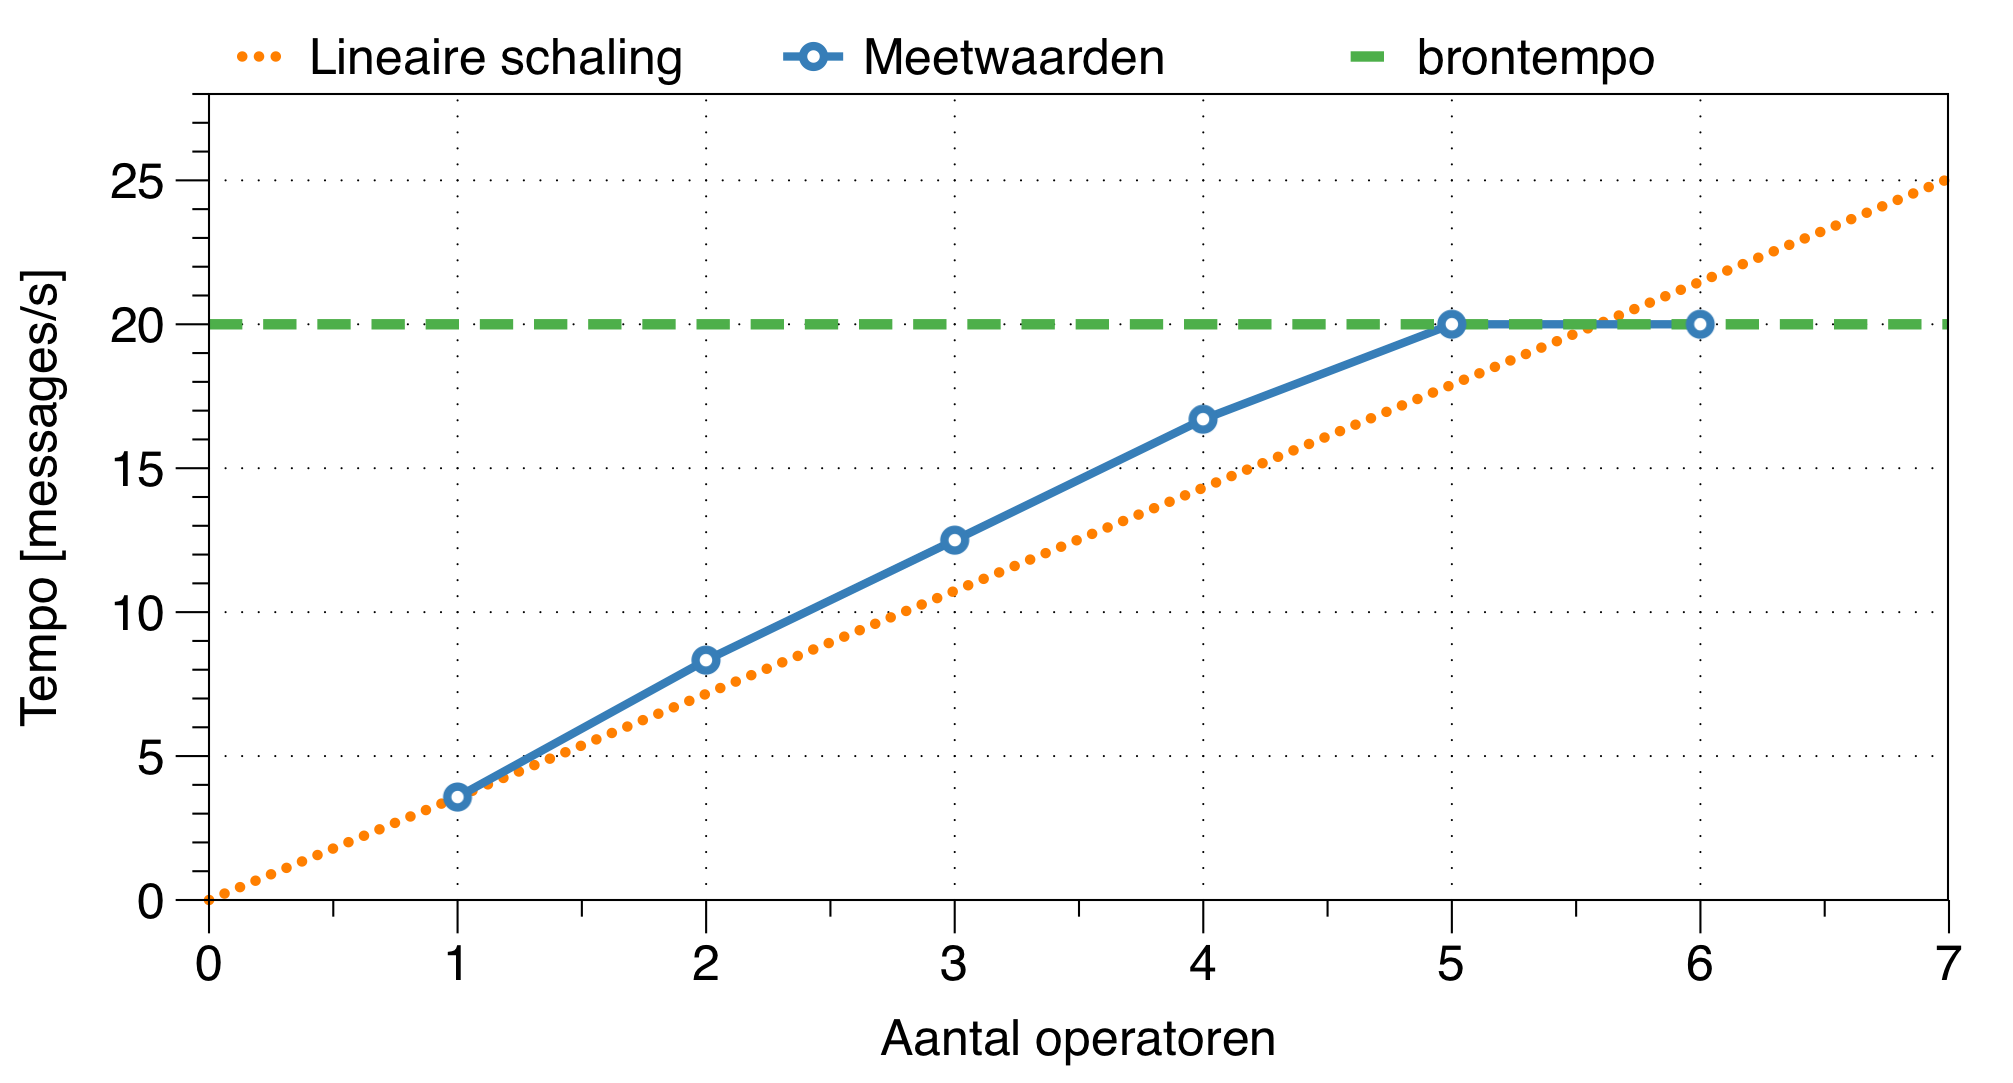
\includegraphics[width=0.49\textwidth]{metingen}
    \caption{Meetwaarden met lineaire schaling.}\label{fig:metingen}
\end{figure}

\begin{table*}[]
    \centering
    \begin{tabular}{@{}llrr@{}}
    \toprule
    Operatoren & Metingen  & Gemiddelde wachttijd [s]                                       & Gemiddelde frequentie [Hz] \\ \midrule
    1          & 500       & $0,2790 $                                              & $3,58$                     \\
    2          & 500       & $0,1200 $                                              & $8,33$                     \\
    3          & 500       & $0,0800$                                             & $12,50$                     \\
    4          & 500       & $0,0599$                                            & $16,70$                     \\
    5          & 500       & $0,0499$                                             & $20,00$                     \\
    6          & 500       & $0,0400$                                             & $20,00$                     \\ \bottomrule
    \end{tabular}
    \caption{Metingen}\label{tab:meaurements}
\end{table*}

Om het systeem te evalueren, wordt het aantal operatoren dat getallen factoriseert geschaald. De source-operator publiceert getallen naar RabbitMQ aan een tempo $f_{s} = 20$ Hz. Deze worden door het systeem verwerkt en gedownload door de sink-operator. Hier worden ze van een timestamp voorzien, waarna later de gemiddelde wachttijd tussen ieder bericht wordt berekend. Dit wordt voor 500 berichten gedaan per meting, waarbij geschaald wordt tot 6 operatoren.

Het resultaat van deze metingen en latere berekeningen is te zien in Tabel~\ref{tab:meaurements} en grafisch in Figuur~\ref{fig:metingen}. Ook is het tempo waarin de bron berichten publiceert weergegeven, waaruit duidelijk valt op te merken dat het systeem afkapt op 20 berichten per seconde. 

Een tweede, interessantere observatie is het verschil tussen de meetwaarden en een lineaire schaling. Deze schaling is een schatting van de verwerkingscapaciteit op basis van de eerste operator. Aangezien een operator aan een gemiddelde frequentie $\overline{f_1} = 3,58$ Hz berichten verwerkt, zou een redelijke schatting kunnen zijn dat dit aantal verdubbelt voor 2 operatoren.

De meetwaarden liggen echter boven deze lineaire schaling, wat gezien bovenstaande redenering dus onverwachts zou kunnen zijn. Dit fenomeen is echter volledig te verklaren door de eerder besproken architectuur; wat nog maar eens de kracht van dit soort systemen in de verf zet.

De generatie van willekeurige nummers genereert zowel nummers die snel gefactoriseerd kunnen worden als nummers waarop langer gerekend moet worden. Bij één operator zullen al deze problemen sequentieel afgehandeld moeten worden, wat de gemiddelde tijd omlaag brengt. Bij meerdere operatoren is echter automatisch \emph{load balancing}. Mocht een operator dus langer moeten rekenen, blijven de andere beschikbaar voor de kortere taken af te handelen.

\newpage

\section{Besluit}
In de voorgaande secties zijn \emph{message brokers}, stream-verwerking en Docker Swarm geïntroduceerd. Op basis van deze technieken is een \emph{distributed stream processing system} geïmplementeerd voor een Raspberry Pi-cluster. 

Om de performantie en schaalbaarheid te evalueren, is gekozen om getallen te factoriseren, waarbij dit de bottleneck vormt. Hiermee zijn dan metingen gedaan voor een variabel aantal operatoren. 

Uit deze metingen blijkt dat het systeem lineair schaalt en nog additionele voordelen heeft van automatische \emph{load balancing}.



\onecolumn

\appendix
\section{Schalen van het aantal transform-operatoren}\label{appendix:schalen}
\begin{minted}{console}
pi@raspberrypi:~/Documents $ sudo docker service ls
ID                  NAME                MODE                REPLICAS            IMAGE               PORTS
z17loeeu5jp8        eloquent_jepsen     replicated          1/1                 filter:latest       
waucpjaqe1g7        silly_hamilton      replicated          2/2                 transform:latest    
pi@raspberrypi:~/Documents $ sudo docker service scale waucpjaqe1g7=3
waucpjaqe1g7 scaled to 3
overall progress: 3 out of 3 tasks 
1/3: running   [==================================================>] 
2/3: running   [==================================================>] 
3/3: running   [==================================================>] 
verify: Service converged 
pi@raspberrypi:~/Documents $ sudo docker service ls
ID                  NAME                MODE                REPLICAS            IMAGE               PORTS
z17loeeu5jp8        eloquent_jepsen     replicated          1/1                 filter:latest       
waucpjaqe1g7        silly_hamilton      replicated          3/3                 transform:latest    
pi@raspberrypi:~/Documents $ 
\end{minted}

\section{Schermafbeelding van RabbitMQ}
\begin{figure*}[htb]
    \centering
    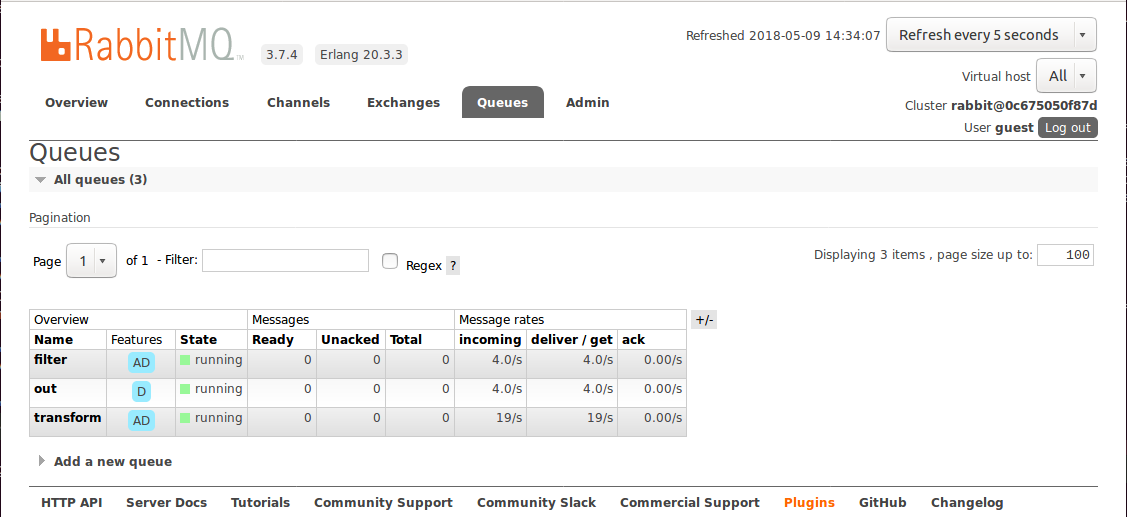
\includegraphics[width=0.9\textwidth]{main_1_2}
    \caption{Screenshot van RabbitMQ met één transform-operator. De filter-queue is de tweede operatie.}\label{fig:dashboard}
\end{figure*}

\newpage

\section{spout.py}
\inputminted[breaklines=true]{python}{code/spout.py}

\section{transform.js}
\inputminted[breaklines=true]{javascript}{code/transform.js}

\section{text.js}
\inputminted[breaklines=true]{javascript}{code/filter.js}


\section{sink.py}
\inputminted[breaklines=true]{python}{code/output.py}

\section{Dockerfile operatoren}
Omwille van een verschillende implementatie van node.js voor ARM of i86, moet er een speciale versie van de Docker container voor node gekozen worden. 
\inputminted[breaklines=true]{docker}{code/Dockerfile}

\section{Metingen}
\begin{figure*}[htb]
    \centering
    \begin{subfigure}{0.88\textwidth}
        \centering
        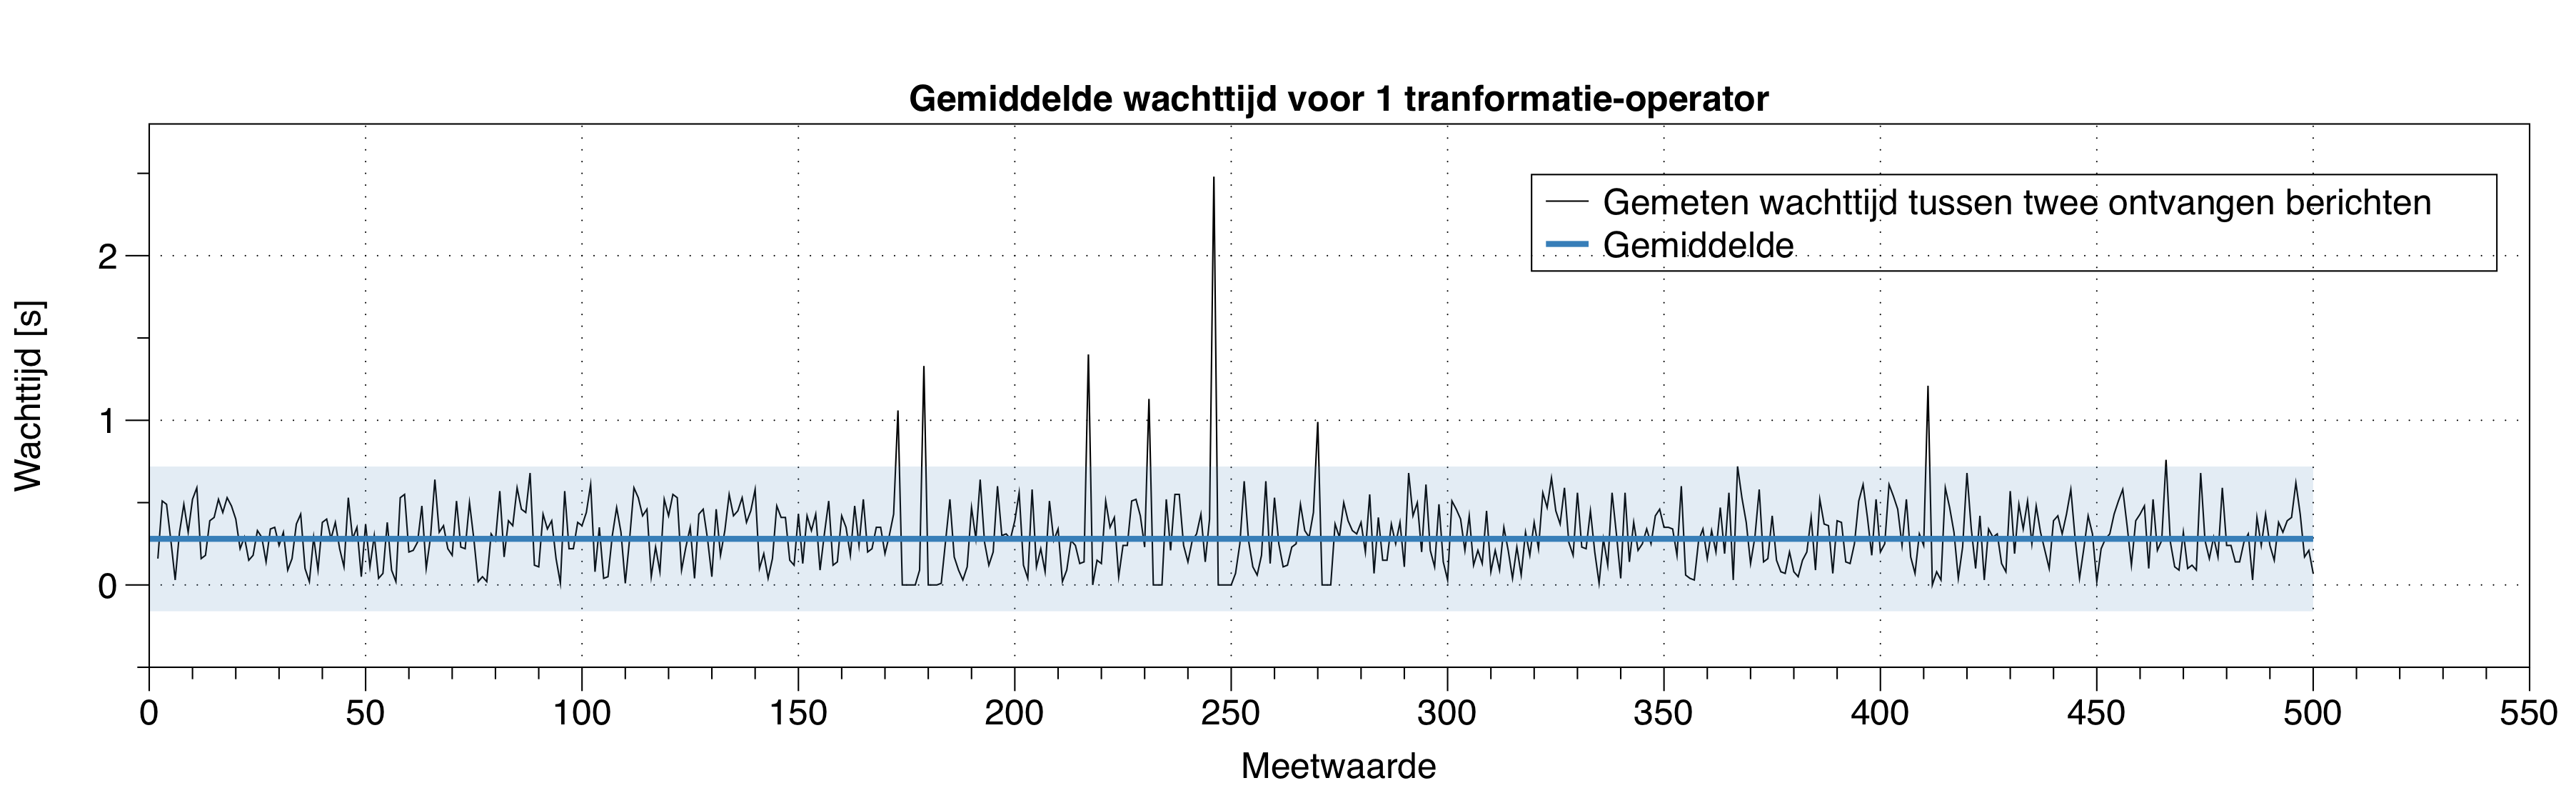
\includegraphics[width=\textwidth]{1_operator}        
    \end{subfigure}  
    \begin{subfigure}{0.88\textwidth}
        \centering
        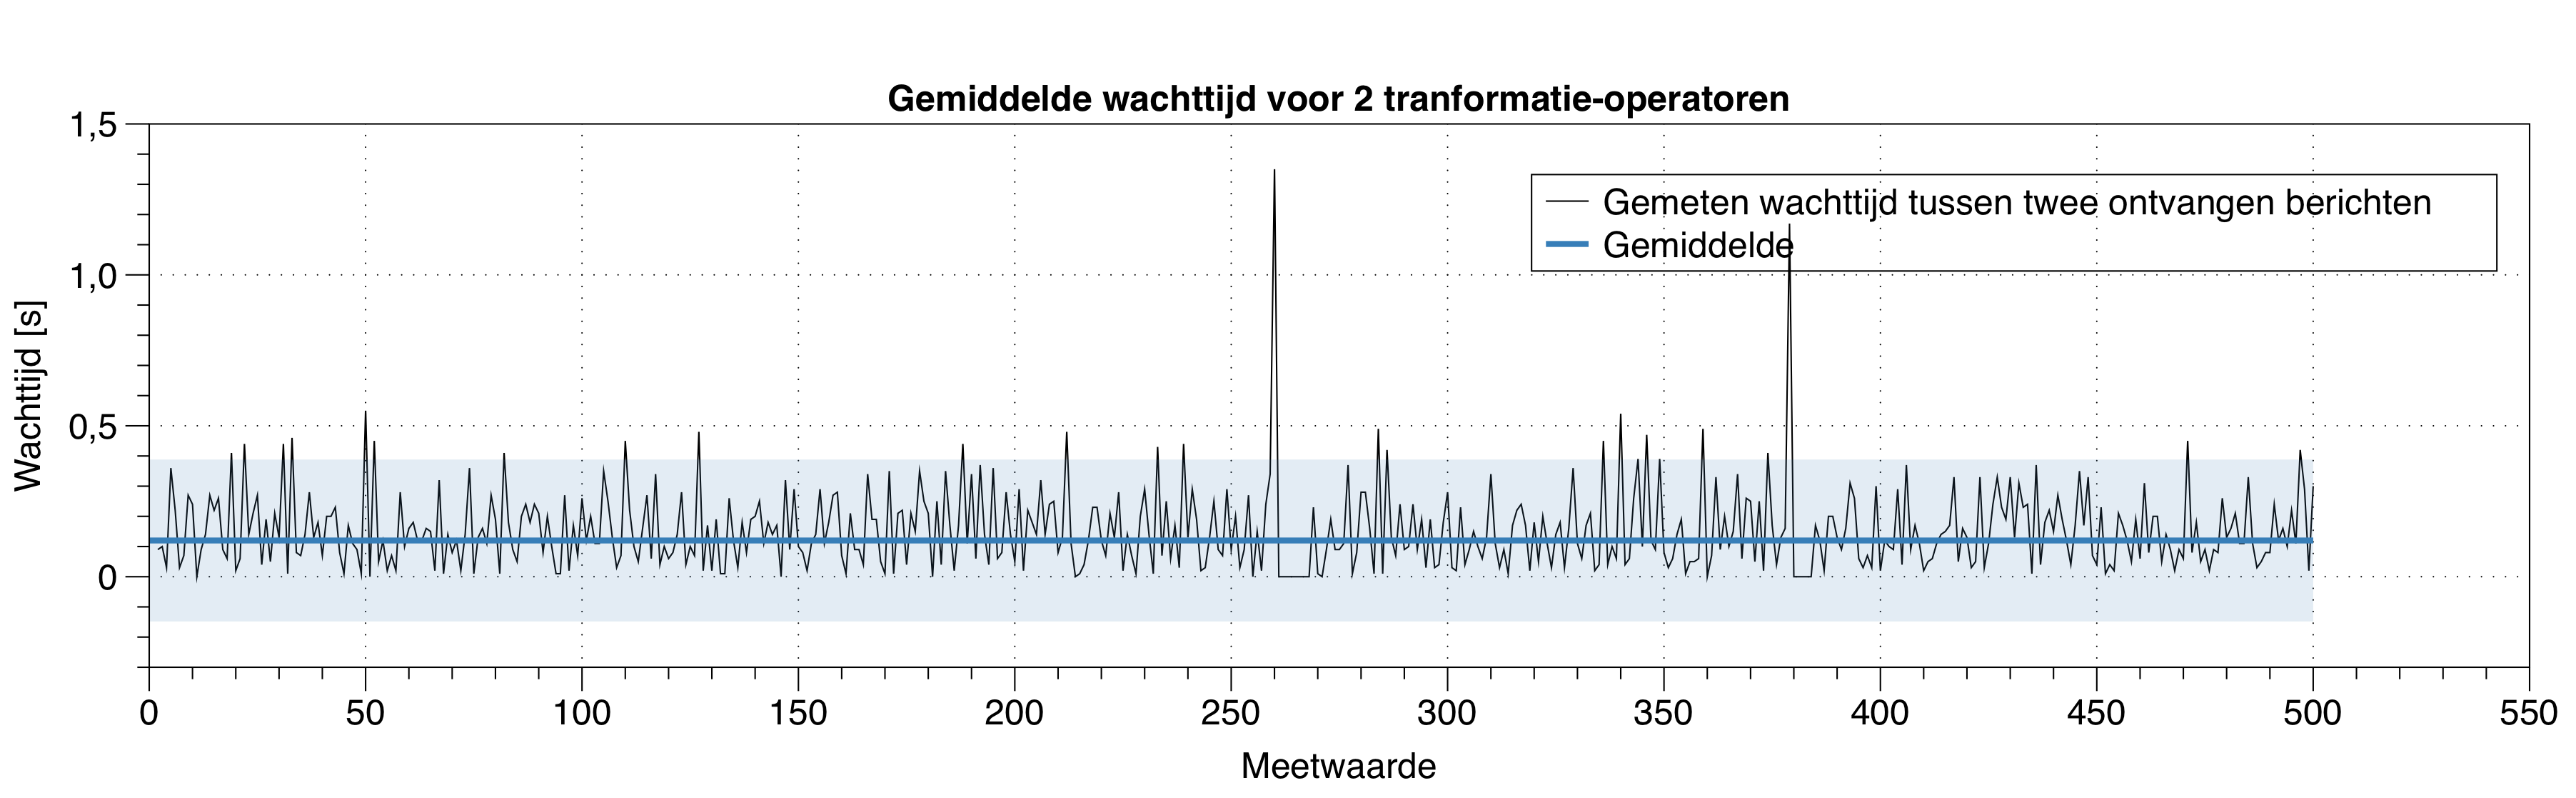
\includegraphics[width=\textwidth]{2_operator}        
    \end{subfigure}  
    \begin{subfigure}{0.88\textwidth}
        \centering
        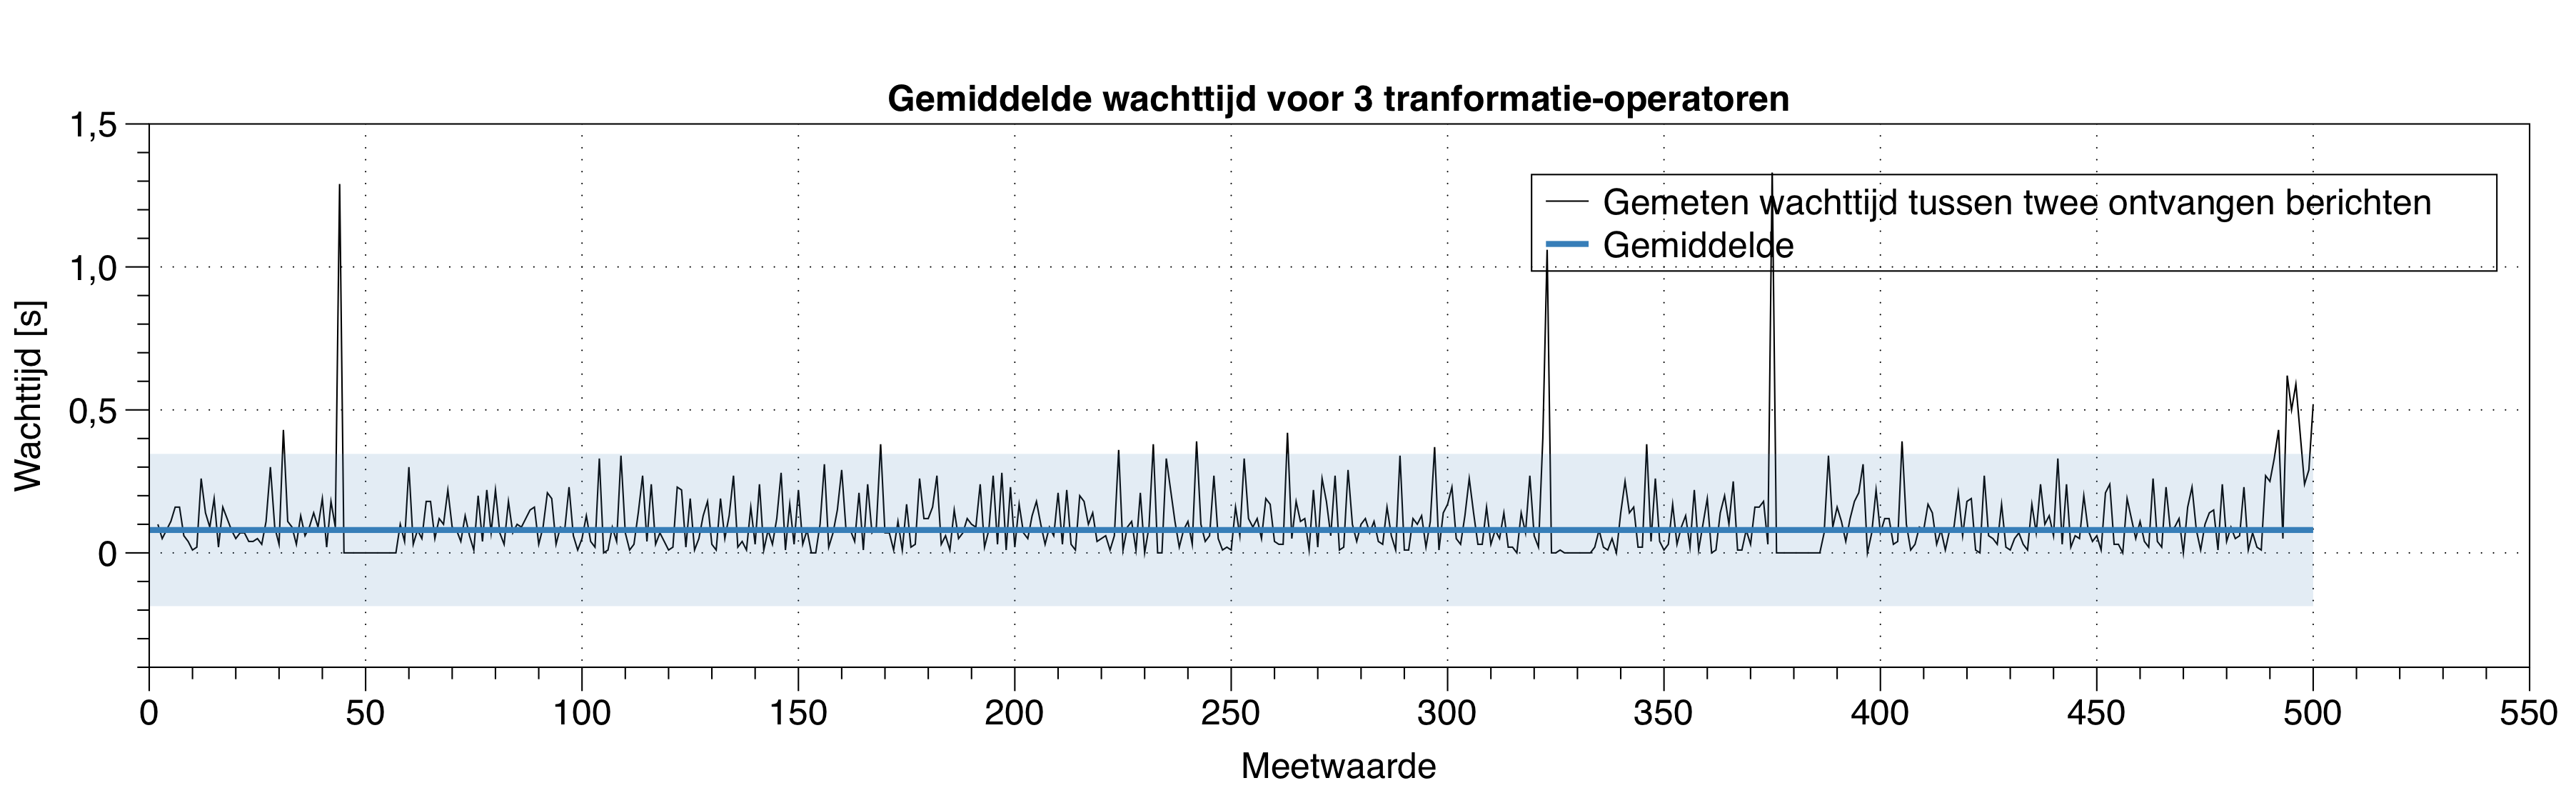
\includegraphics[width=\textwidth]{3_operator}        
    \end{subfigure}  
    \begin{subfigure}{0.88\textwidth}
        \centering
        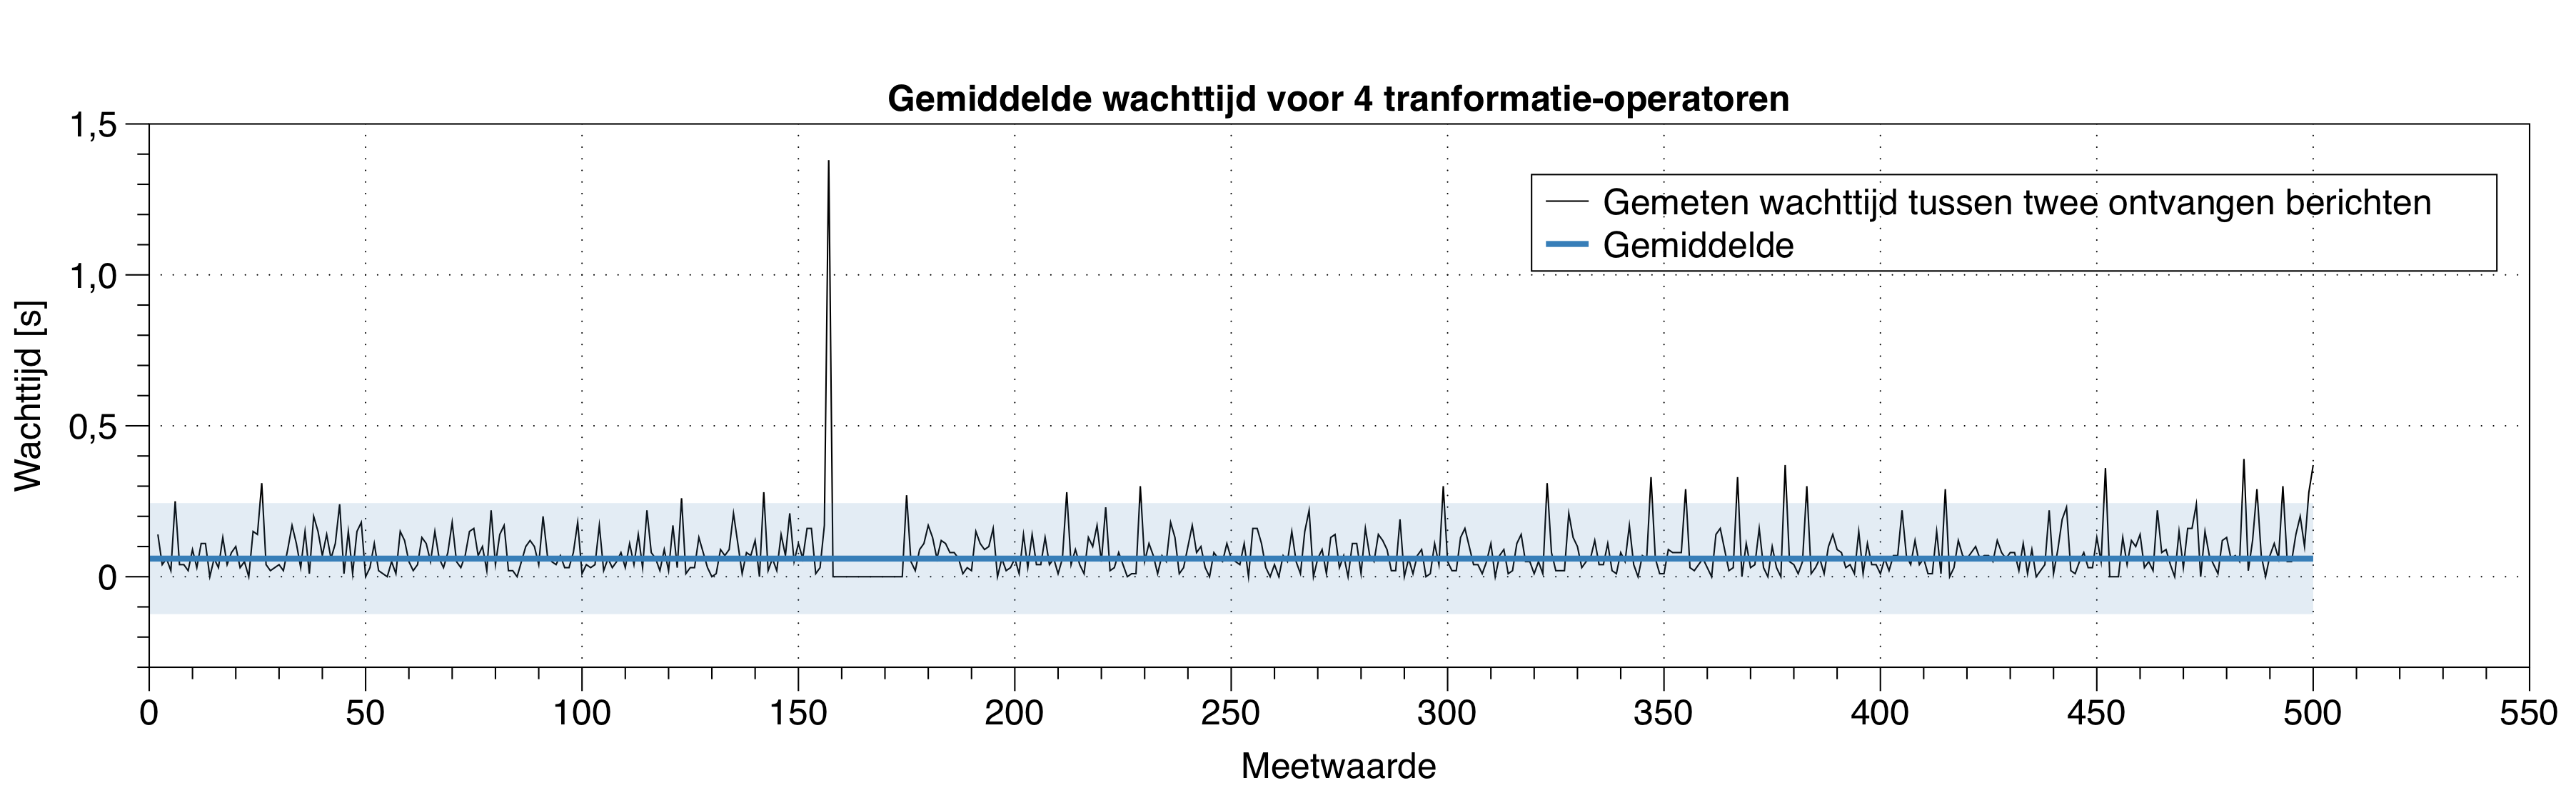
\includegraphics[width=\textwidth]{4_operator}        
    \end{subfigure}
    \begin{subfigure}{0.88\textwidth}
        \centering
        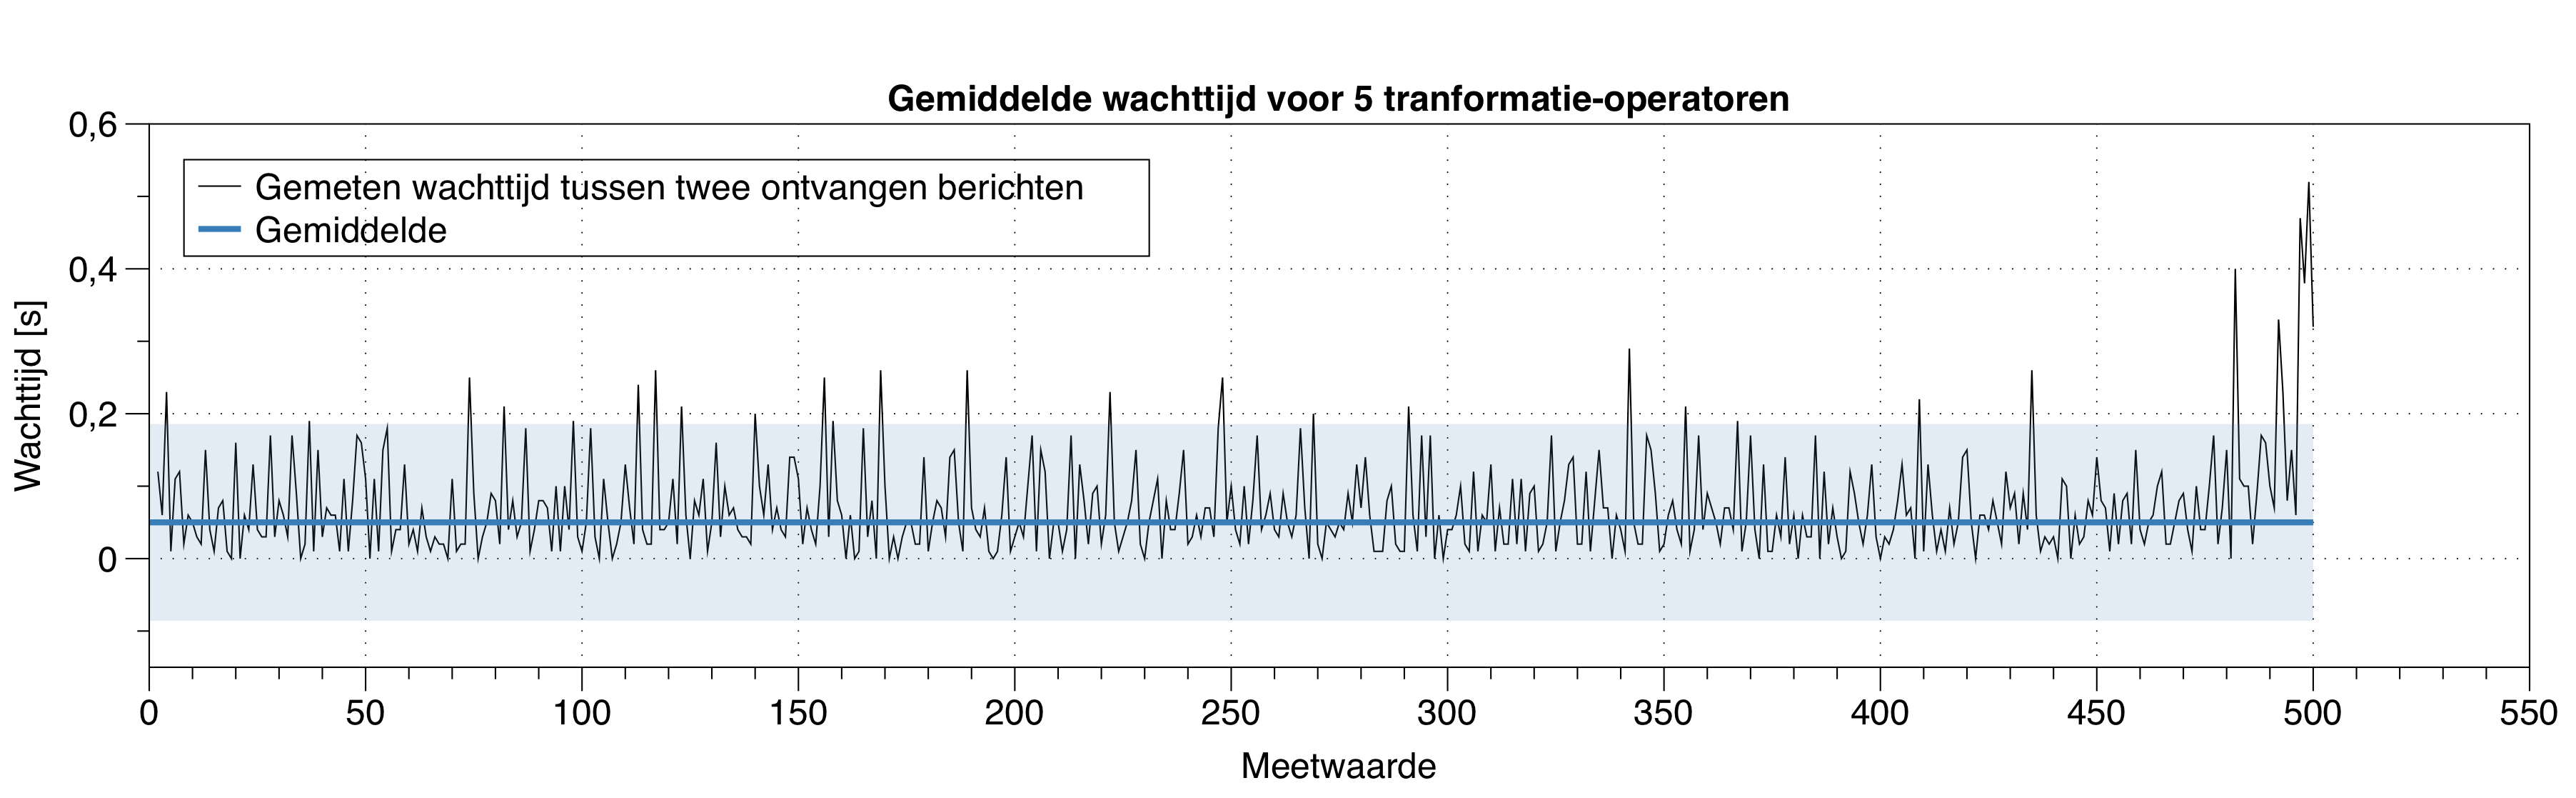
\includegraphics[width=\textwidth]{5_operator}        
    \end{subfigure}  
\end{figure*}

\newpage

% The appendix command is issued once, prior to all appendices, if any.
%\appendix
\end{document}
